% Intended LaTeX compiler: pdflatex
\documentclass[a4paper,10pt]{jarticle}
\usepackage{amsmath, amssymb, bm}
\usepackage[dvipdfmx]{graphicx}
\usepackage[dvipdfmx]{color}
\usepackage{times}
\usepackage{longtable}
\usepackage{minted}
\usepackage{fancyvrb}
\setlength{\oddsidemargin}{-.1in}
\setlength{\evensidemargin}{-.1in}
\setlength{\topmargin}{-4em}
\setlength{\textwidth}{6.5in}
\setlength{\textheight}{10in}
\setlength{\parskip}{0em}
\setlength{\topsep}{0em}
\setlength{\columnsep}{3zw}
\usepackage{coins-EngA-jp}
\advisor{櫻井哲也 (コンピュータサイエンス専攻)}
\gakuseki{201611350}
\heiseiyear{30}
\majorfield{知能情報メディア主専攻}
\year{2018}
\month{8}
\day{3}
\usepackage{ascmac}
\author{江畑 拓哉}
\date{}
\title{情報科学類専門語学A}
\begin{document}

\maketitle
\section{文献}
\label{sec:org8aaf515}
Lars Elde ́n., Matrix Methods in Data Mining and Pattern Recognition., SIAM, 2007.\\
\section{概要}
\label{sec:orgd18daa0}
 ``Matrix Methods in Data Mining and Pattern Recognition'' は行列の固有値分解などの基礎的な手法からパターン認識やデータマイニングなどの問題に対する解法について説明されている文献である。今回はその中でも第1部である chapter1 から chapter9 までを取り上げて輪講を行った。以下はその内自分が担当した内容について説明したものである。\\
\section{Chapter 5 QR 分解}
\label{sec:org244e2db}
 QR分解 という行列の圧縮手法がある。これは、ある行列 \(\bm{A}\) を直交行列と三角行列に因数分解する手法である。これは2つの要素が両方共三角行列であることだけが要求されるという点で、LU分解よりも広い範囲をカバーしている。\footnote{LU分解には分解する行列が正則であるという適用条件がある。}\\
\subsection{直交変換を用いた三角行列への変換}
\label{sec:orgdefcfb8}
 直交変換の一つであるハウスホルダー変換を用いることで、任意の行列 \(\bm{A} \in \mathbb{R}^{m\times n}\ where\ m\geq n\) について上三角行列 \(\bm{R}\) と直交行列 \(\bm{Q} \in \mathbb{R}^{m \times m}\) を用いた関係式を作ることが出来る。\\
\begin{align*}
\bm{A}\rightarrow \bm{Q}^T \bm{A} = 
\begin{pmatrix}\bm{R} \\ \bm{0}\end{pmatrix}
&& where\ \bm{R}\ \in\ \mathbb{R}^{n\times n}
\end{align*}
 以下に具体的に分解を行った例を示す。\\

\textbf{\(\bm{A}\in\mathbb{R}^{5\times 4}\) である場合}\\
 最初のステップでは1列目の上から1番目より下の要素をゼロにする。\\
\begin{align*}
\bm{H}_1\bm{A} = \bm{H}_1
\begin{pmatrix}
\times & \times & \times & \times \\
\times & \times & \times & \times \\
\times & \times & \times & \times \\
\times & \times & \times & \times \\
\times & \times & \times & \times \\
\end{pmatrix}
=
\begin{pmatrix}
+ & + & + & + \\
0 & + & + & + \\
0 & + & + & + \\
0 & + & + & + \\
0 & + & + & + \\
\end{pmatrix}
\end{align*}
 \(+\) の値は \(\times\) に対して変形が行われ値が変わっているという事を示している。直交行列である \(\bm{H}_1\) の適用は、ハウスホルダー変換を行うことに等しい。\\
 次のステップでは変換した \(\bm{A}\) に対して、前のステップと同様に2列目の上から2番目より下の要素をゼロにして、\\
\begin{align*}
\bm{H}_2
\begin{pmatrix}
\times & \times & \times & \times \\
0 & \times & \times & \times \\
0 & \times & \times & \times \\
0 & \times & \times & \times \\
0 & \times & \times & \times \\
\end{pmatrix}
=
\begin{pmatrix}
\times & \times & \times & \times \\
0 & + & + & + \\
0 & 0 & + & + \\
0 & 0 & + & + \\
0 & 0 & + & + \\
\end{pmatrix}
\end{align*}
 三番目のステップでも同様に変換して、\\
\begin{align*}
\bm{H}_3
\begin{pmatrix}
\times & \times & \times & \times \\
0 & \times & \times & \times \\
0 & 0 & \times & \times \\
0 & 0 & \times & \times \\
0 & 0 & \times & \times \\
\end{pmatrix}
=
\begin{pmatrix}
\times & \times & \times & \times \\
0 & \times & \times & \times \\
0 & 0 & + & + \\
0 & 0 & 0 & + \\
0 & 0 & 0 & + \\
\end{pmatrix}
\end{align*}
 四番目のステップでも同様にして、上三角行列 \(\bm{R}\) を得ることが出来る。\\
 この変換を要約すると、\\
\begin{align*}
\bm{Q}^T\bm{A}=
\begin{pmatrix}
\bm{R} \\
\bm{0}
\end{pmatrix}
&& where\ \bm{Q}^T =\bm{H}_4\bm{H}_3\bm{H}_2\bm{H}_1
\end{align*}
 また、 \(\bm{H}_i\ where\ \bm{A}\ \in\ \mathbb{R}^{m\times n}\) の構造は以下のようになる。\\
\begin{align*}
\bm{H}_1 &= \bm{I} - 2\bm{u}_1\bm{u}_1^T && where\ \bm{u}_1\ \in\ \mathbb{R}^m \nonumber \\
\bm{H}_2 &= 
\begin{pmatrix}
1 & 0 \\
0 & \bm{P}_2
\end{pmatrix}
&& where\ \bm{P}_2=\bm{I} - 2\bm{u}_2\bm{u}_2^T,\ \bm{u}_2\ \in\ \mathbb{R}^{m-1}
\nonumber \\ 
\bm{H}_3 &= 
\begin{pmatrix}
1 & 0 & 0 \\
0 & 1 & 0 \\
0 & 0 & \bm{P}_3 
\end{pmatrix}
&& where\ \bm{P}_3=\bm{I} - 2\bm{u}_3\bm{u}_3^T,\ \bm{u}_3\ \in\ \mathbb{R}^{m-2}
\end{align*}
 このようにして、単位行列に連続して小さくなっていくハウスホルダー変換を埋め込んでいき、それと同時にベクトル \(\bm{u}_i\) の次元も小さくなる。\\
\subsection{QR 分解}
\label{sec:org8f0f31f}
\begin{itembox}[l]{Theorem 5.1 QR分解}
 どのような行列 $\bm{A}\ where\ \bm{A}\ \in\ \mathbb{R}^{m\times n},\ m \geq n$ についても直交行列によって上三角行列に変形することが出来る。またこの変形は以下の行列の圧縮に等しい。

\begin{align*}
\bm{A} = \bm{Q}
\begin{pmatrix}
\bm{R}\\
\bm{0}
\end{pmatrix}&& where\ &\bm{Q}\ \in\ \mathbb{R}^{m\times m}\ is\ orthogonal \\
             &&& \bm{R}\ \in\ \mathbb{R}^{n\times n}\ is\ upper\ triangular
\end{align*}
(orthogonal matrix=直交行列,upper triangular matrix=上三角行列)
 もし $\bm{A}$ が列について線形独立であるならば $\bm{R}$ は正則である。
\end{itembox}
\begin{itembox}[l]{Proof}
 単位ベクトルに変換されるベクトルがゼロベクトルであれば選ばれた直交変換が恒等行列に等しい、という条件のもとで、一般的なケースに適用することは容易である。
 以下の行列の列について線形独立性を考える。
\begin{align*}
\begin{pmatrix}
\bm{R} \\
\bm{0}
\end{pmatrix}
\end{align*}
 $\bm{R}$ は上三角行列であることから、線形独立性より対角成分は非ゼロ。(もし対角成分にゼロがある場合には、その列の左側の列との線型結合があると言える) そして $\bm{R}$ の行列式が非ゼロならば、 $\bm{R}$ は正則である。
\end{itembox}

 QR 分解を抽象的に示すと、以下のようになる。\\
\begin{figure}[htbp]
\centering
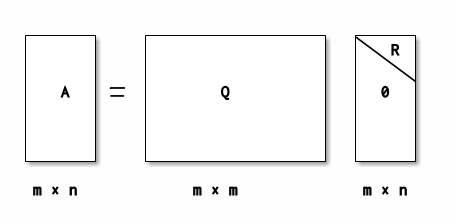
\includegraphics[width=.9\linewidth]{../chapter5/figure5-1.png}
\caption{QR分解の図}
\end{figure}

 Aの列の直交化に対応するQの部分のみを用いる代替手段は分解を行う際にしばしば有用である。その薄いQR分解は \(\bm{Q} = (\bm{Q}_1\bm{Q}_2)\ where\ \bm{Q}_1\ \in\ \mathbb{R}^{m\times n}\) に分割することで行われる。 \(\bm{Q}_2\) が0に掛けられても 0 となることに注意しなければならない。\\

\begin{figure}[htbp]
\centering
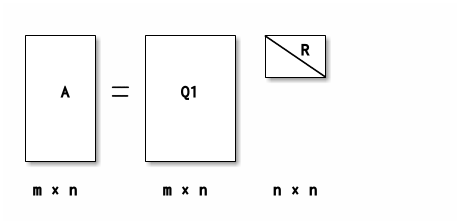
\includegraphics[width=.9\linewidth]{../chapter5/figure5-2.png}
\caption{薄いQR分解の図}
\end{figure}

\begin{align*}
\bm{A} = (\bm{Q}_1\bm{Q}_2)\begin{pmatrix}\bm{R}\\0\end{pmatrix}=\bm{Q}_1\bm{R}
\end{align*}
 この方程式から、 \(\bm{R}(\bm{A})=\bm{R}(\bm{Q}_1)\) がわかる。以上で値空間 \(\bm{R(A)}\) の直交基底を計算したことになる。更に上式において j 列を書き出すと、\\
\begin{align*}
\bm{a}_j = \bm{Q}_1\bm{r}_j = \Sigma^j_{i = 1}r_{ij}\bm{q}_i
\end{align*}
 \(\bm{R}\) の j 列は直交基底の \(\bm{a}_j\) の位置を保持することがわかる。\\

\textbf{Example 5.2 単純な数を用いた QR 分解}\\

 以下に Octave (Matlab) での QR 分解の実行を示す。\\
\textbf{Octave Code}\\
\begin{minted}[frame=lines,linenos=true,obeytabs,tabsize=4]{octave}
A = [1 1 1;
     1 2 4; 
     1 3 9;
     1 4 16];
[Q,R] = qr(A)
\end{minted}
\textbf{Output}\\
\begin{minted}[frame=lines,linenos=true,obeytabs,tabsize=4]{text}
Q =

  -0.50000   0.67082   0.50000   0.22361
  -0.50000   0.22361  -0.50000  -0.67082
  -0.50000  -0.22361  -0.50000   0.67082
  -0.50000  -0.67082   0.50000  -0.22361

R =

   -2.00000   -5.00000  -15.00000
    0.00000   -2.23607  -11.18034
    0.00000    0.00000    2.00000
    0.00000    0.00000    0.00000

\end{minted}

薄いQR分解は \(qr(A,0)\) コマンドで実行する。\\

\textbf{Octave Code}\\
\begin{minted}[frame=lines,linenos=true,obeytabs,tabsize=4]{octave}
A = [1 1 1;
     1 2 4; 
     1 3 9;
     1 4 16];
[Q,R] = qr(A,0)
\end{minted}

\textbf{Output}\\
\begin{minted}[frame=lines,linenos=true,obeytabs,tabsize=4]{text}
Q =

  -0.50000   0.67082   0.50000
  -0.50000   0.22361  -0.50000
  -0.50000  -0.22361  -0.50000
  -0.50000  -0.67082   0.50000

R =

   -2.00000   -5.00000  -15.00000
    0.00000   -2.23607  -11.18034
    0.00000    0.00000    2.00000

\end{minted}
\subsection{最小二乗問題}
\label{sec:org2ec464e}
 QR分解を用いて、以下の最小二乗問題を 正規方程式 \footnote{\(\bm{A}^T\bm{A}\bm{x} = \bm{A}^T\bm{b}\)}を形成することなく解くことが出来る。これを行うために、ユークリッドベクトルノルムは直交変換の元で変わらないという事実を利用する。\\
\begin{align}
\min_{x}||\bm{b}-\bm{A}\bm{x}||_2&&where\ \bm{A}\ \in\ \mathbb{R}^{m\times n},\ m\geq n
\end{align}
\begin{align*}
||\bm{Q}\bm{y}||_2=||\bm{y}||_2  
\end{align*}
 残差ベクトルに A についてのQR分解を用いて、\\
\begin{align*}
||\bm{r}||_2^2&=||\bm{b}-\bm{A}\bm{x}||_2^2=||\bm{b}-\bm{Q}\begin{pmatrix}\bm{R}\\0\end{pmatrix}\bm{x}||^2_2 \\
&=||\bm{Q}(\bm{Q}^T\bm{b}-\begin{pmatrix}\bm{R}\\0\end{pmatrix}\bm{x})||^2_2=||\bm{Q}^T\bm{b}-\begin{pmatrix}\bm{R}\\0\end{pmatrix}\bm{x}
||^2_2
\end{align*}
 ここで \(\bm{Q}=(\bm{Q}_1\ \bm{Q}_2),\ where\ \bm{Q}_1\ \in\ \mathbb{R}^{m\times n}\) と分割して以下の式を導く。\\
 \begin{align*}
\bm{Q}^T\bm{b}=\begin{pmatrix}\bm{b}_1\\\bm{b}_2\end{pmatrix}:=\begin{pmatrix}\bm{Q}^T_1\bm{b}\\\bm{Q}^T_2\bm{b}\end{pmatrix}
\end{align*}
 即ち残差ベクトルの式は以下のように変形できる。\\
\begin{align}
||\bm{r}||^2_2=||\begin{pmatrix}\bm{b}_1\\\bm{b}_2\end{pmatrix}-\begin{pmatrix}\bm{R}\bm{x}\\0\end{pmatrix}||^2_2=||\bm{b}_1-\bm{R}\bm{x}||^2_2+||\bm{b}_2||^2_2
\tag{1}
\end{align}

 さらに A が線形独立であると仮定した場合、以下の式を満たす値を求めることで \(||\bm{r}||_2\) を最小化する値を求めることが出来る。\\
\begin{align*}
\bm{R}\bm{x}=\bm{b}_1
\end{align*}
 ここで次の定理が成り立つことになる。\\
\begin{itembox}[l]{Theorem 5.3 QR分解を用いた最小二乗問題の解}
 列についてフルランクであり、QR分解によって $\bm{A}=\bm{Q}_1\bm{R}$ となる行列 $\bm{A}\ \in\ \mathbb{R}^{m\times n}$ の最小二乗問題 $min_x||\bm{A}\bm{x}-\bm{b}||_2$ は以下の唯一解を持つ。
\begin{align*}
\bm{x}=\bm{R}^{-1}\bm{Q}_1^T\bm{b}
\end{align*}
\end{itembox}


\textbf{Example 5.4 QR分解を用いて最小二乗問題を解く}\\

 以下に Octave (Matlab) での QR 分解を用いた最小二乗問題の解法を示す。\\
 尚 MATLAB では \(x=A\backslash b\) とすると同じアルゴリズムで解を求めることが出来る。\\

\textbf{Octave Code}\\
\begin{minted}[frame=lines,linenos=true,obeytabs,tabsize=4]{octave}
A = [1 1;
     1 2; 
     1 3;
     1 4;
     1 5];
b = [7.9700;
     10.2000;
     14.2000;
     16.0000;
     21.2000];
# thin QR
[Q1,R]=qr(A,0)
x=R\(Q1'*b)
\end{minted}

\textbf{Output}\\
\begin{minted}[frame=lines,linenos=true,obeytabs,tabsize=4]{text}
Q1 =
  -4.4721e-01  -6.3246e-01
  -4.4721e-01  -3.1623e-01
  -4.4721e-01   2.7756e-17
  -4.4721e-01   3.1623e-01
  -4.4721e-01   6.3246e-01
R =
  -2.23607  -6.70820
   0.00000   3.16228
x =
   4.2360
   3.2260
\end{minted}

\section{Chapter 7 Krylov 部分空間法}
\label{sec:org39cd53f}
 次元削減を行うための手法として打ち切りSVD(Truncated SVD)や PCR(主成分回帰)を用いることがあるが、分解後の右辺の残差を減らすように基底を選択出来る手法として Lanczos-Golub-Kahan (LGK) 二重対角化がある。\\
 LGK 二重対角化は線形代数の分野で用いられていおり、 Lanczos 二重対角化とも呼ばれる。また計量科学やその他の分野では部分的最小二乗法(PLS(Partial Least Squares/Projection Latent structures))に密接して関連した方法として知られている。Krylov 部分空間法 の中から来た手法であり、疎な線形問題(sparse linear systems)や、固有値・特異値の計算で用いられる。\\
 Krylov 部分空間法は再帰的であるが、始めに導出としてハウスホルダー変換を用いて行列を二重対角化する手法を扱う。\\
\subsection{ハウスホルダー変換を用いた二重対角化}
\label{sec:org34d8ecc}
密行列 \(\bm{C}\in\mathbb{R}^{m\times(n+1)}\) の SVD を計算するアルゴリズムの最初のステップは、左から右へハウスホルダー変換をし、上二重対角の形に \(\bm{C}\) を変換することである。\\
 \(m > n\) を仮定すると、以下の形が求まる。\\

\begin{align*}
\bm{C} &= \bm{P}\begin{pmatrix}\hat{\bm{B}}\\\bm{0}\end{pmatrix}\bm{W}^T\\
where\ \bm{P}, \bm{W} \ &is\ orthogonal\\
      \hat{\bm{B}} \ &is\ upper bidiagonal
\end{align*}
 この自己圧縮は \(\Rightarrow\) 疎・密行列の最小二乗問題の近似解を求める際などでも有用である。\\
例として、 \(\bm{C}\in\mathbb{R}^{6 \times 5}\) を用いて説明する。※ \(m = 6,\ n + 1 = 5\)\\
まず 1 列目の非対角成分を、左側からかける変換行列 \(\bm{P}^T_1\in\mathbb{R}^{6\times6}\) を用いて 0 にする。\\

\begin{align*}
\bm{P}^T_1 \bm{C} = \bm{P}^T_1
\begin{pmatrix}
\times & \times & \times & \times & \times \\
\times & \times & \times & \times & \times \\
\times & \times & \times & \times & \times \\
\times & \times & \times & \times & \times \\
\times & \times & \times & \times & \times \\
\times & \times & \times & \times & \times
\end{pmatrix}
=
\begin{pmatrix}
\ast & \ast & \ast & \ast & \ast \\
0 & \ast & \ast & \ast & \ast \\
0 & \ast & \ast & \ast & \ast \\
0 & \ast & \ast & \ast & \ast \\
0 & \ast & \ast & \ast & \ast \\
0 & \ast & \ast & \ast & \ast 
\end{pmatrix}
\end{align*}
 次に、別の右からかける変換行列 \(\bm{W}_1\) を用いて 1 行目の 3 番目の要素から右側をすべて 0 にする。 \(\bm{W}_1\) は以下のように表すことができる。\\
\begin{align*}
\mathbb{R}^{5\times5} \ni \bm{W}_1 = 
\begin{pmatrix}
1 & \bm{0} \\
\bm{0} & \bm{Z}_1 
\end{pmatrix}
where\ \bm{Z}_1\ &is\ Householder\ transformation
\end{align*}
 これを用いた変換は 1 列目の要素に対しては何も影響しない。つまり前に行った 1 列目の非対角成分を 0 にした変換の効果は打ち消されない。結果は以下のようになる。\\
\begin{align*}
\bm{P}^T_1\bm{C}\bm{W}_1 =
\begin{pmatrix}
\times & \times & \times & \times & \times \\
0 & \times & \times & \times & \times \\
0 & \times & \times & \times & \times \\
0 & \times & \times & \times &  \times \\
0 & \times & \times & \times &  \times \\
0 & \times & \times & \times &  \times
\end{pmatrix}
\bm{W}_1
=
\begin{pmatrix}
\times & \ast & 0 & 0 & 0 \\
0 & \ast & \ast & \ast & \ast \\
0 & \ast & \ast & \ast & \ast \\
0 & \ast & \ast & \ast &  \ast \\
0 & \ast & \ast & \ast &  \ast \\
0 & \ast & \ast & \ast &  \ast
\end{pmatrix}
=: \bm{C}_1
\end{align*}
 同様の手法を用いて 2 列目の対角成分よりも下の成分を 0 にする変換行列 \(\bm{P}_2\) を \(\bm{C}_1\) にかける 。但し 1 行目の要素については値が変わらないようにする。\\
 すると、 \(\bm{P}_2\) は以下のように表すことができる。\\
\begin{align*}
\mathbb{R}^{6\times 6} \ni \bm{P}_2 =
\begin{pmatrix}
1 & \bm{0}\\
\bm{0} & \tilde{\bm{P}_2}
\end{pmatrix}
where\ \tilde{\bm{P}_2} \in \mathbb{R}^{5\times5}\ is\ Householder\ transformation
\end{align*}
 これを適用して、\\
\begin{align*}
\bm{P}^T_2\bm{C}_1 = 
\begin{pmatrix}
\times & \times & 0 & 0 & 0\\ 
0 & \ast & \ast & \ast & \ast\\
0 & 0 & \ast & \ast & \ast\\
0 & 0 & \ast & \ast & \ast\\
0 & 0 & \ast & \ast & \ast\\
0 & 0 & \ast & \ast & \ast\\
\end{pmatrix}
\end{align*}
 そして同様に右からかける変換行列 \(\bm{W}_2\) は以下のように表すことができる。\\
\begin{align*}
\bm{W}_2 =
\begin{pmatrix}
\bm{I}_2 & \bm{0}\\
\bm{0} & \bm{Z}_2 
\end{pmatrix}
,\ 
\bm{I}_2 = 
\begin{pmatrix}
1 & 0 \\
0 & 1
\end{pmatrix}
\end{align*}
 これも \(\bm{W}_1\) 同様 \(\bm{P}_2\) で 0 にした部分を汚すことなく 2 列目の 4行目以降の要素を0にする。\\
\begin{align*}
\bm{P}^T_2\bm{C}_1\bm{W}_2 = 
\begin{pmatrix}
\times & \times & 0 & 0 & 0 \\  
0 & \times & \ast & 0 & 0 \\
0 & 0 & \ast & \ast & \ast \\
0 & 0 & \ast & \ast & \ast \\
0 & 0 & \ast & \ast & \ast \\
0 & 0 & \ast & \ast & \ast \\
\end{pmatrix}
=: \bm{C}_2
\end{align*}
 この操作を繰り返すことで最終的に以下の形を得る。\\
\begin{align*}
\bm{P}^T\bm{C}\bm{W} &=
\begin{pmatrix}
\times & \times & & & \\
 & \times & \times& & \\
 & & \times & \times &  \\
&&&\times & \times  \\
&&&& \times   \\
&&&&& \\
\end{pmatrix}
=
\begin{pmatrix}
\hat{\bm{B}}\\
\bm{0}
\end{pmatrix} \\
where\ \bm{P} &= \bm{P}_1 \bm{P}_2 \cdots \bm{P}_n \in \mathbb{R}^{m \times m}\\
\bm{W} &= \bm{W}_1 \bm{W}_2 \cdots \bm{W}_{n-1} \in \mathbb{R}^{(n+1)\times(n+1)}
 \tag{2}
\end{align*}

 一般的に上で示された \(\bm{P}\) , \(\bm{W}\) はハウスホルダー変換の積であり、\\
\begin{align*}
\hat{\bm{B}} =
\begin{pmatrix}
\beta_1& \alpha_1& & & \\
&\beta_2& \alpha_2&  & \\
&&\ddots& \ddots &   \\
&&& \beta_n& \alpha_n   \\
&&&& \beta_{n+1}   \\
\end{pmatrix}
\in \mathbb{R}^{(n+1)\times(n+1)}
\end{align*}

 は上二重対角行列である。\\
 これらは、この章の残りの部分で用いられる直交行列を生成するための構造を持っている。\\
\begin{itembox}[l]{Proposition 7.3}
 二重対角分解 (2) 式における $\bm{P}$ の列を $\bm{p}_i,i=1,2,\dots,m$ として表すと以下のように表すことが出来る。
\begin{align*}
\bm{p}_1 = \bm{\beta}_1 \bm{c}_1,\ \bm{W} = 
\begin{pmatrix}
1 & \bm{0}\\
\bm{0} & \bm{Z}
\end{pmatrix}
\ where\ \bm{Z}\in\mathbb{R}^{n \times n}\ is\ orthogonal
\end{align*}
$c_1$ は $\bm{C}$ の最初の列である。
\end{itembox}
\begin{itembox}[l]{Proof}
  $i = 1$ の場合は、 $\bm{P}^T \bm{c}_1 = \beta_1 \bm{e}_1$ であったことから明らかである。これ以降の場合では、 $\bm{W}_i$ が以下の構造で表されていたことからわかる。
\begin{align*}
\bm{W}_i &=
\begin{pmatrix}
\bm{I}_i & \bm{0}\\
\bm{0} & \bm{Z}_i 
\end{pmatrix} \\
where\ \bm{I}_i &\in \mathbb{R}^{i \times i}\ is\ identicaly\ matrices \\
\bm{Z}_i &are \ orthogonal
\end{align*}
\end{itembox}

 ハウスホルダー変換を用いた二重対角化への削減は \(4mn^2 - 4n^3 / 3\) flopsかかる。\\
もし \(m \gg n\) ならば、 \(\bm{A}\) を上三角行列にして、 \(\bm{R}\) 要素を二重対角化したほうが良い。\footnote{R とは LU 分解で言う U 要素(LU 分解の別名は LR分解)}\\

 最小二乗問題 \(\min_x||\bm{b}-\bm{A}\bm{x}||_2,\ where\ \bm{A}\in\mathbb{R}^{m\times n}\) を解く場合について考える。\\
 二重対角化において \(\bm{C} = (\bm{b}\  \bm{A})\) とした場合、同等の二重対角化最小二乗問題(bidiagonal least squares problem)を得ることが出来る。式(3) と命題 7.3 より以下を得る。\\
\begin{align*}
\bm{P}^T\bm{C}\bm{W} = \bm{P}^T
\begin{pmatrix}
\bm{b} & \bm{A}
\end{pmatrix}
\begin{pmatrix}
1 & \bm{0}\\
\bm{0} & \bm{Z}
\end{pmatrix}
=
\begin{pmatrix}
\bm{P}^T\bm{b}& \bm{P}^T\bm{A}\bm{Z}
\end{pmatrix}
=
\begin{pmatrix}
\beta_1 & \bm{B}\\
\bm{0} & \bm{0}
\end{pmatrix} \tag{3}
\end{align*}
\begin{align*}
&where \\
&\bm{B} =
\begin{pmatrix}
 \alpha_1& & & \\
\beta_2& \alpha_2&  & \\
&\ddots& \ddots &   \\
&& \beta_n& \alpha_n   \\
&&& \beta_{n+1}   \\
\end{pmatrix}
\in \mathbb{R}^{(n+1)\times n}
\end{align*}
 そして \(\bm{y} = \bm{Z}^T\bm{x}\) として残差の 2 ノルムを以下のように書くことができる。\\
\begin{align*}
||\bm{b} - \bm{A}\bm{x}||_2 &=
|| \begin{pmatrix}
\bm{b} & \bm{A}
\end{pmatrix}
\begin{pmatrix}
1 \\
-\bm{x}
\end{pmatrix}||_2 = 
||
\bm{P}^T
\begin{pmatrix}
\bm{b} & \bm{A}
\end{pmatrix}
\begin{pmatrix}
1 & \bm{0} \\
\bm{0} & \bm{Z}
\end{pmatrix}
\begin{pmatrix}
1 \\ - \bm{y}
\end{pmatrix}
||_2 \\
&= ||
\begin{pmatrix}
\bm{\bm{P}^T\bm{b}} & \bm{P}^T\bm{A}\bm{X}
\end{pmatrix}
\begin{pmatrix}
1 \\
-\bm{y}
\end{pmatrix}
||_2 =
|| \beta_1\bm{e}_1 - \bm{B}\bm{y}||_2 \tag{4}
\end{align*}
 もし平面回転の操作によって \(\bm{B}\) が上二重対角行列に変換される場合、この二重対角最小二乗問題 \(\min_y||\beta_1\bm{e}_1 - \bm{B}\bm{y}||_2\) は \(O(n)\) flopsで解くことが出来る。\\
\subsection{LGK 二重対角化}
\label{sec:org3581da6}
 ここでは前で述べた二重対角化手法ではない別の手法を扱う。この手法は式(3)の計算を再帰的に解く。これを LGK 二重対角化 という。式(3)の最後の式は以下のように書くことが出来る。\\
\begin{align*}
\bm{P}^T\bm{A}=
\begin{pmatrix}
\bm{B}\bm{Z}^T\\
\bm{0}
\end{pmatrix}  where \ \bm{B}\bm{Z}^T \in \mathbb{R}^{(n+1)\times n}
\end{align*}
 これは更に詳しく書けば以下のようになる。\\
\begin{align*}
&\bm{A}^T
\begin{pmatrix}
\bm{p}_1& \bm{p}_2&\cdots & \bm{p}_{n+1}
\end{pmatrix}
= \bm{Z} \bm{B}^T  \\
&= 
\begin{pmatrix}
\bm{z}_1 & \bm{z}_2 &\cdots &\bm{z}_n
\end{pmatrix}
\begin{pmatrix}
\alpha_1& \beta_2& & & & &&\\
&\alpha_2& \beta_3&  & &&&\\
&&\ddots& \ddots &   &&&\\
&&&& \beta_i &&\\
&&&& \alpha_i && \\
&&&&&\ddots & \ddots & \\ 
&&&&&& \alpha_n & \beta_{n+1}   \\
\end{pmatrix}
\end{align*}
 両辺の \(i\) 列 \((i\geq 2)\) を比較すると以下のような式が考えられる。\\
\begin{align*}
\bm{A}^T\bm{p}_i = \beta_i\bm{z}_{i-1} + \alpha_i \bm{z}_i
\end{align*}
 変形して\\
\begin{align*}
\alpha_i\bm{z}_i=\bm{A}^T\bm{p}_i - \beta_i\bm{z}_{i-1} \tag{5}
\end{align*}
 同様に \(i\) 列について、 \((\bm{P}\bm{P}^T\bm{A}\bm{Z}=\bm{P}\bm{B}\bm{Z}^T\bm{Z})\)\\
\begin{align*}
&\bm{A}\bm{Z}
= \bm{A}
\begin{pmatrix}
\bm{z}_1 & \bm{z}_2 & \cdots & \bm{z}_n
\end{pmatrix} \\ 
&= \bm{P}\bm{B} = 
\begin{pmatrix}
\bm{p}_1 & \bm{p}_2 & \cdots & \bm{p}_{n+1}
\end{pmatrix}
\begin{pmatrix}
\alpha_1 &&&&&&& \\
\beta_2 & \alpha_2 &&&&&& \\
& \ddots & \ddots &&&&&\\
&&&& \alpha_i &&& \\
&&&& \beta_{i+1} &&& \\
&&&&&& \ddots & \ddots &\\
&&&&&&& \beta_n & \alpha_n \\
&&&&&&&& \beta_{n+1}
\end{pmatrix}
\end{align*}
 同様に以下のような式が考えられる。\\
\begin{align*}
\bm{A}\bm{z}_i = \alpha_i\bm{p}_i + \beta_{i+1}\bm{p}_{i+1}
\end{align*}
 変形して\\
\begin{align*}
\beta_{i+1}\bm{p}_{i+1}=\bm{A}\bm{z}_i -\alpha_i\bm{p}_i \tag{6}
\end{align*}

等式 \(\beta_1\bm{p}_1 = \bm{b}\) を初期値として等式(5), (6)を再帰的に解くことが出来る。\\

\begin{center}
\begin{tabular*}{\linewidth}{l}
\hline
\textbf{LGK 二重対角化}\\
\hline
1. \(\beta_1\bm{p}_1 = \bm{b}, \bm{z}_0 = 0\)\\
2. \(for\ i\ =\ 1\ :\ n\)\\
$\backslash$ $\backslash$ $\backslash$ \(\alpha_i\bm{z}_i = \bm{A}^T\bm{p}_i-\beta_i\bm{z}_{i-1}\)\\
$\backslash$ $\backslash$ $\backslash$ \(\beta_{i+1}\bm{p}_{i+1} = \bm{A}\bm{z}_i- \alpha_{i}\bm{p}_i\)\\
3. end\\
\\
\hline
\end{tabular*}
\end{center}


 係数 \(\alpha_{i-1}, \beta_i\) は \(||\bm{p}_i|| = ||\bm{z}_i||=1\) となるように決定する。\\

 再帰の終点は \(\alpha_i\) 又は \(\beta_i\) がゼロと等しくなったときである。最小二乗問題の解法においてこれは明確に定義されている特別な場合であることがわかっているので、終点とみなしても問題がない。\\
 正確な算術手続きを考えれば、再帰的二重対角化の手続きはハウスホルダー変換を用いた二重対角化と等しくなる。従ってこの過程で生成された \((\bm{p_i})^n_{i=1}\) \((\bm{z}_i)^n_{i=1}\) は \(\bm{p}_i^T\bm{p}_j=0 ,\ \bm{z}_i^T\bm{z}_j=0\ if\ i\neq j\) を満たす。\\
 しかし浮動点計算を考慮すると、生成されるベクトルは再帰の過程で直交性を失ってしまう。\\
\section{Chapter 9 非負行列の因数分解}
\label{sec:org21b7147}
 ある行列 \(\bm{A}\in\mathbb{R}^{m\times n}\) が与えられ、非負の要素を持ように制限された \(k\) ランクの近似を行いたいと考えた時、言い換えれば \(\bm{W}\in\mathbb{R}^{m\times k}\) と \(\bm{H}\in\mathbb{R}^{k\times n}\) を仮定して以下の式を解きたい場合について考える。\\
\begin{align*}
\min_{\bm{W}\geq 0, \bm{H}\geq 0}&||\bm{A}-\bm{W}\bm{H}||_F\\  \tag{7}
where\ ||\bm{A}||_F &= \sqrt{\Sigma_i\Sigma_j|a_{ij}|^2}\ means\ Frobenius\ norm
\end{align*}
 同時に \(\bm{W}\) と \(\bm{H}\) を最適化しようとした時、この問題は非線形になる。\\
 しかし、行列の一つが既にわかっている場合、例えば \(\bm{W}\) がわかっている場合で言えば、この \(\bm{H}\) を求める問題は、非負の制限がついた右側の行列についての最小二乗問題であると言える。\\
 従って元の問題に対する最も一般的な解決法は、交互最小二乗法 (ALS) を使うことである。\\
\subsection{Alternating nonnegative least squares のアルゴリズム}
\label{sec:org06de0d9}
\begin{itembox}[l]{Alternating nonnegative least squares algorithm}
1. 初期値 $\bm{W}^{(1)}$ を与える。
2. $k = 1 , 2 \dots$ と収束するまで繰り返す。
    - $\min_{H\geq0} ||\bm{A}-\bm{W}^{(k)}\bm{H}||_F$ を解き、 $\bm{H}^{(k)}$ を得る
    - $\min_{W\geq0} ||\bm{A}-\bm{W}\bm{H}^{(k)}||_F$ を解き、 $\bm{W}^{(k+1)}$
\end{itembox}

 しかし、近似 \(\bm{W}\bm{H}\) は単一のものではない。ここで正の対角要素を持つ任意の対角行列 \(\bm{D}\) とその逆行列を要素間に適用しすることが出来る。\\
\begin{align*}
\bm{W}\bm{H} = (\bm{W}\bm{D})(\bm{D}^{-1}\bm{H})
\end{align*}
 ある要素の増大と他の要素の減衰を防ぐために、毎反復ごとにそれらの一つを正規化する必要がある。一般的な正規化は、 \(\bm{W}\) の各列の最大要素が \(1\) になるように \(\bm{W}\) の列をスケーリングすることである。\\
  \(\bm{A}\) と \(\bm{H}\) の列要素として、 \(\bm{a_j}\) と \(\bm{h_j}\) を置く。各行の要素を一つずつ書き下すと、この最小二乗問題は以下の \(n\) 個の独立したベクトルの最小二乗問題と等しいものとみなすことが出来る。\\
\begin{align*}
\min_{h_j\geq 0}||\bm{a}_j - \bm{W}^{(k)}\bm{h}_j||_2 \ where\ j= 1,2,\dots , n
\end{align*}
 この行列を転置することで、 \(\bm{W}\) を決定するの最小二乗問題は、独立な \(m\) このベクトルの最小二乗問題に変換される。即ち ALS アルゴリズムのコア部分は擬似的なMATLABコードで以下のように表すことが出来る。\\

\textbf{疑似 MATLAB コード}\\
\begin{minted}[frame=lines,linenos=true,obeytabs,tabsize=4]{matlab}
while (not converged)
    [W] = normalize(W);
    for i = 1:n
        H(;,i) = lsqnonneg(W, A(:,i));
    end
    for i = 1:m
        w = lsqnonneg(W, A(:, i));
        W(i,:) = w';
    end
end
\end{minted}

 非負値行列因子分解のためのアルゴリズムは多くの種類がある。前頁のアルゴリズムは、非負な最小二乗法のためのアクティブセット法にかなり時間がかかってしまうという欠点がある。より簡易な代替手段として、部分QR分解 \(\bm{W}=\bm{Q}\bm{R}\) を用いることで非負という制約がない最小二乗解を得ることが出来る。そして \(\bm{H}\) におけるすべての負の要素はゼロと等しいとみなすことが出来る。これは \(\bm{W}\) の計算においても同様の議論をすることが出来る。\\
\begin{align*}
\bm{H} = \bm{R}^{-1}\bm{Q}^T\bm{A}
\end{align*}

\textbf{疑似 MATLAB コード (上の例に基づけば \(\bm{V} = \bm{A}\))}\\
\begin{minted}[frame=lines,linenos=true,obeytabs,tabsize=4]{matlab}
while (not converged)
    W = W.*(W >= 0);
    H = H.*(W'*V)./((W'*W)*H+epsilon);
    H = H.*(H>=0);
    W = W.*(V*H')./(W*(H*H')+epsilon);
    [W,H] = normalize(W, H);
end
\end{minted}

  \(epsilon\) は極小の値であり、これはゼロ除算を避けるために用いられている。 .\(\ast\) や .\(\slash\) で表される行列操作はそれぞれの構成要素についての演算で、\\
\begin{align*}
\bm{H}_{ij} := \bm{H}_{ij}
\frac{(\bm{W}^T\bm{A})_{ij}}{{(\bm{W}^T\bm{W}\bm{H})_{ij}+\epsilon}},\ \bm{W}_{ij} := \bm{W}_{ij}\frac{(\bm{A}\bm{H}^T)_{ij}}{{(\bm{W}\bm{H}\bm{H}^T)_{ij}+ \epsilon}}
\end{align*}
 尚このアルゴリズムは勾配降下法と考えることが出来る。\\
 非負値行列分解には非常に多くの重要な用途があるため、これのアルゴリズム開発は活発に行われている。例えば、反復法を用いた終了基準を見つける問題は未だ良い解決策を見つけたとは言い難い。\\
 非負値行列分解 \(\bm{A}\approx \bm{W}\bm{H}\) はクラスタリングにも用いられている。各データを表すベクトル \(\bm{a}_j\) は、もし \(\bm{h}_{ij}\) が \(\bm{H}\) の \(j\) 列の最大の要素であるなら、それはクラスタ \(i\) に割り当てられる。\\
 さらにこの分解法は文書分類、電子メールの監視\footnote{楽譜にすること}、バイオインフォマティクス、スペクトル分析のような分野でも用いられている。\\
\subsection{初期化}
\label{sec:orgcfb858c}
 非負値行列分解のアルゴリズムにはいくつかの問題がある。それは全体での最適解が求まる保証がないということである。このアルゴリズムではしばしば収束が遅いことや順最適解 (厳密解ではない) になってしまうことがある。良好な初期の近似を計算するための効率的な手法として、 \(A\) の SVD に基づいて行うというものがある。最初の \(k\) 個の特異の三つの組 \((\bm{\sigma}_i,\bm{u}_i,\bm{v}_i)^k_{i=1}\) は、フロベニウスノルムにおいて \(A\) の最適なランク \(k\) の近似を与える。\\
 もし \(A\) が非負な行列であったならば、 \(\bm{u}_i\) や \(\bm{v}_1\) が非負であることは明らか。(Section 6.4)\\
 つまりもし \(\bm{A} =\bm{U}\bm{\Sigma}\bm{V}^T\) が \(\bm{A}\) の SVD であるならば、特異ベクトル \(\bm{u}_1\) を \(\bm{W}^{(1)}\) の最初の列であるとすることが出来る。 (同様に以降のアルゴリズムのため、 \(\bm{v}_1^T\) を初期近似 \(\bm{H}^{(1)}\) の 第1行 であるする。)\\
 次の最良なベクトル \(\bm{u}_2\) は直交性が満たされているために負の成分を有する可能性が非常に高い。しかし行列 \(\bm{C}^{(2)} = \bm{u}_2\bm{v}_2^T\) を計算しすべての負の成分をゼロにすることで非負な行列 \(\bm{C}^{(2)}_+\) を得ると、この行列の最初の特異ベクトルは非負であることがわかる。さらにそれは、これが \(\bm{u}_2\) の合理的で良い近似であると考えることが出来るので、 \(\bm{W}^{(1)}\) の第2列として取り上げることが出来る。\\
 前頁の手続きを MATLAB を使って簡潔に書き下すと以下のようになる。 \footnote{\([\bm{U},\bm{S}, \bm{V}]\) = svds (A, k) は Lanczos 法を用いることで、k 個の最大特異値及び対応する特異ベクトルとを計算する。標準なSVD関数である \(svd(A)\) はすべての分解を計算するがこれはかなり遅く、特に行列が大きな疎行列のときはより遅くなる。}\\

\textbf{MATLAB Code}\\
\begin{minted}[frame=lines,linenos=true,obeytabs,tabsize=4]{matlab}
[U,S,V] = svds (A, k) % Compute only the k largest singular
W (:,1) = U (:,1);    % values and the corresponding vectors
for j = 2:k
    C = U (:,j)*V (:,j)';
    C = C .* (C>=0);
    [u, s, v] = svds (C, 1);
    W (:,j) = u;
end
\end{minted}

\textbf{Example 9.4}\\
 ランク2 の行列 \(\bm{A}\) の非負値分解の例を図3に示す。ここでは初期化をランダムな値で行ったものと、 SVD ベースで行ったものを比較している。ランダムな値で初期化したものは収束がより遅くなており、10回反復させても収束したとは言い難い。これに対してSVD ベースで初期化したものの相対近似誤差は \(0.574\) であることがわかる。 (尚 k-means 法においてこの誤差は \(0.596\) であった)  更にいくつかのケースでランダムに初期化したものは最適でない準最適な値に収束してしまった。\\

\begin{figure}[htbp]
\centering
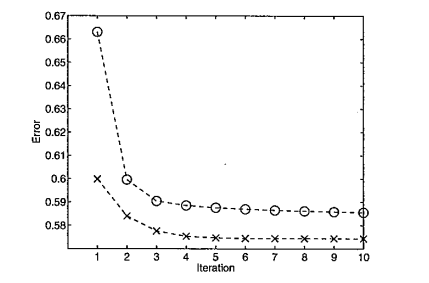
\includegraphics[width=.9\linewidth]{../chapter9/fig9-3.png}
\caption{反復回数を横軸とした相対近似誤差のグラフ。上のカーブは初期化をランダムに行ったもの、下のカーブは SVD ベースで初期化を行ったものである。}
\end{figure}

 SVD ベースの初期化をするこの分解は具体的に以下のようになった。\\
\begin{align*}
\bm{W}\bm{H} = 
\begin{pmatrix}
0.3450 & 0 \\
0.1986 & 0 \\
0.1986 & 0 \\
0.6039 & 0.1838 \\
0.2928 & 0 \\
0 & 0.5854 \\
1.0000 & 0.0141 \\
0.0653 & 1.0000 \\
0.8919 & 0.0604 \\
0.0653 & 1.0000 
\end{pmatrix}
\begin{pmatrix}
0.7740 & 0 & 0.9687 & 0.9120 & 0.5251 \\
0 & 1.0863 & 0.8214 & 0 & 0
\end{pmatrix}
\end{align*}

 前頁のそれは分解の処理を打ち切ることが出来る。最初の四つの文書は基底ベクトルによって表されており、これは Google-related keywords のための大きな要素を持っている。これに対して最後の文書は1つめの基底ベクトルによって表されているが、この座標値は先述の四つの文書に比べて小さくなっている。\\
 この手法では、ランク2の近似は Google-related contents を強調するが、 "football-document" は強調しない。\\

 対して、ランク3の近似を計算した時には以下の値を得ることが出来る。\\
  \(\bm{W}\) の三番目のベクトルは、本質的に "football" についての基底であり、その一方で他の2つのベクトルはGoogle-related document を示している基底である。\\
\begin{align*}
\bm{W}\bm{H} =
&\begin{pmatrix}
0.2516 & 0 & 0.1633 \\
0 & 0 & 0.7942 \\
0 & 0 & 0.7942 \\
0.6924 & 0.1298 & 0 \\
0.3786 & 0 & 0 \\
0 & 0.5806 & 0 \\
1.0000 & 0 & 0.0444 \\
0.0589 & 1.0000 & 0.0007 \\
0.4237 & 0.1809 & 1.0000 \\
0.0589 & 1.0000 & 0.0007  
\end{pmatrix}\\
&\begin{pmatrix}
1.1023 & 0 & 1.0244 & 0.8045 & 0 \\
0 & 1.0815 & 0.8315 & 0 & 0 \\
0 & 0 & 0.1600 & 0.3422 & 1.1271 
\end{pmatrix}
\end{align*}
\end{document}
